\subsubsection{Biểu đồ số phép so sánh}

Đầu tiên, tiến hành vẽ tất cả biểu đồ trên các thứ tự khác nhau của 11 thuật toán, được hình \ref{fig:all_the_number_of_comparisons_for_each_algorithm_of_each_data_order}.

\begin{figure}[H]
    \centering
    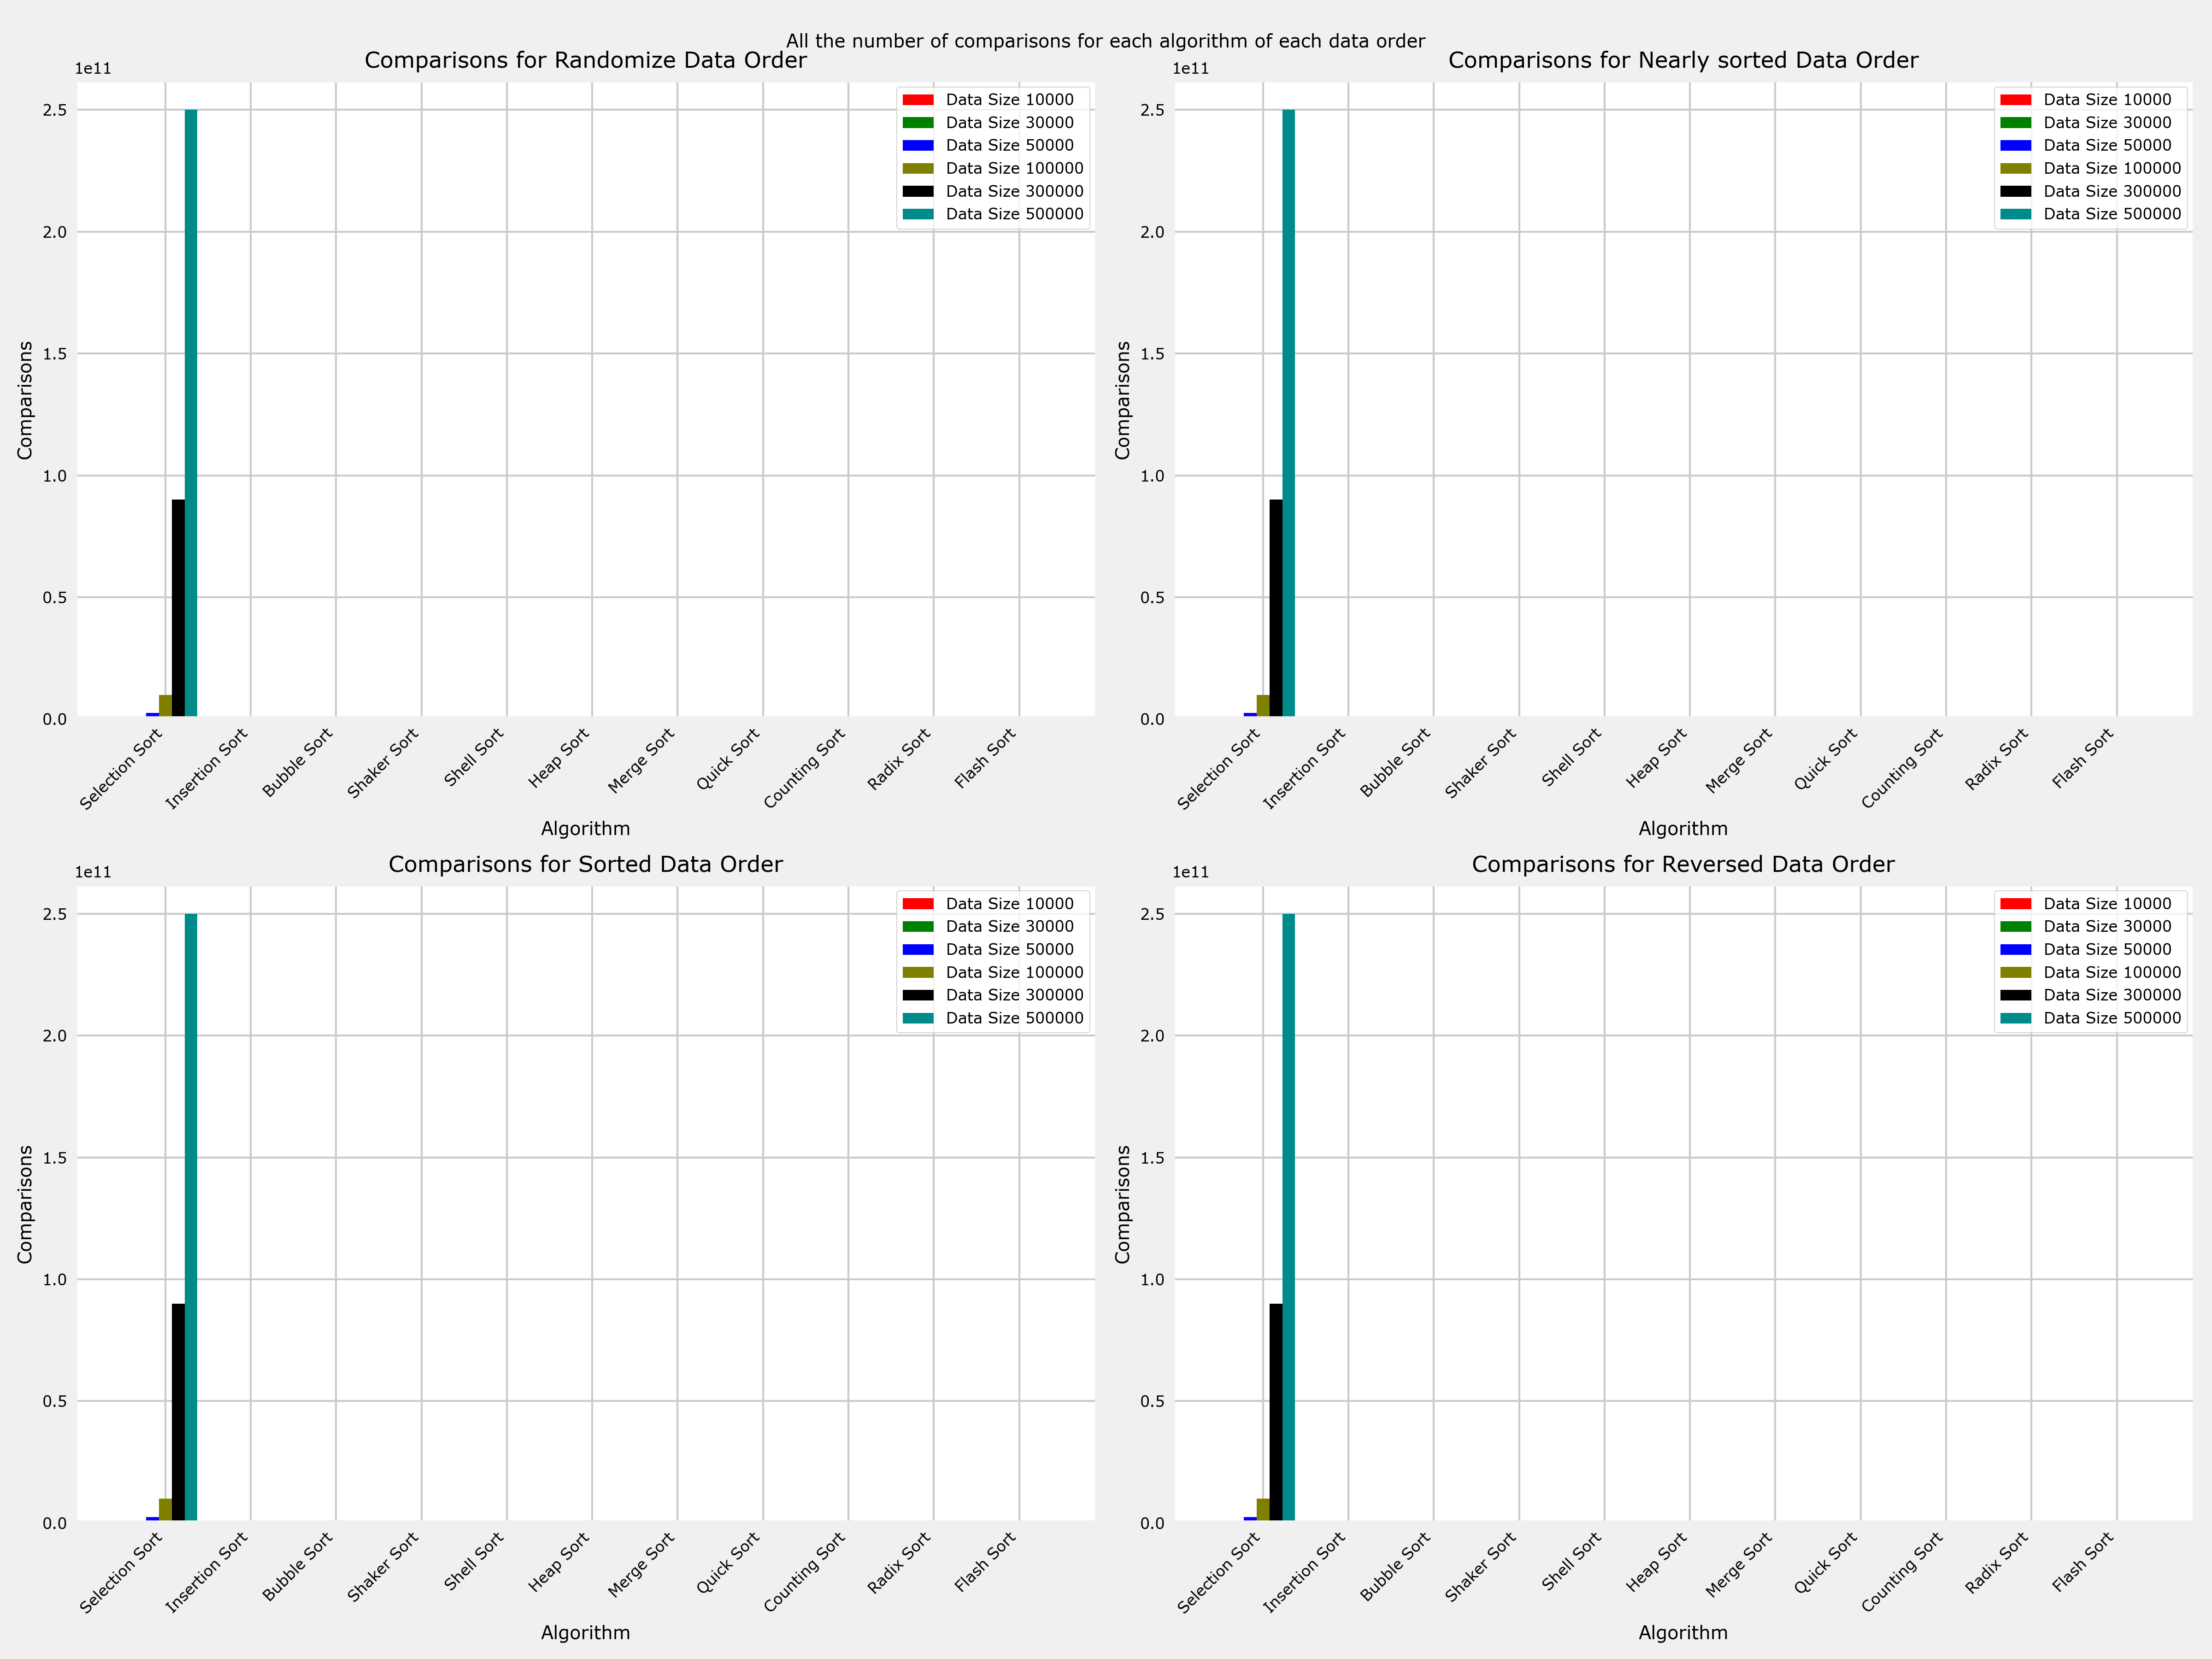
\includegraphics[width=\textwidth]{experimental_result/images/all_the_number_of_comparisons_for_each_algorithm_of_each_data_order.png}
    \caption{Số phép so sánh của 11 thuật toán với tất cả trường hợp của dữ liệu}
    \label{fig:all_the_number_of_comparisons_for_each_algorithm_of_each_data_order}
\end{figure}

Dễ thấy, Selection Sort số lượng phép so sánh vượt trội hơn 10 thuật toán còn lại, và đạt đến 2500049999 phép so sánh. Do đó, các thuật toán còn lại không thể nhìn thấy được trên biểu đồ. Selection Sort tăng rất mạnh khi gặp kích thước dữ liệu tăng dần, thể hiện độ phức tạp thời gian trung bình $\Theta(n^2)$. Vì thuật toán này luôn duyệt tất cả trường hợp có thể xảy ra, không dừng sớm khi đã sắp xếp xong nên số lượng phép so sánh là như nhau đối với tất cả trường hợp của mảng trong thực nghiệm (Phần \ref{subsec:experimental_result}).  

Từ đây bỏ qua Selection Sort để thuận tiện cho việc trực quan hóa dữ liệu.


\begin{figure}[H]
    \centering
    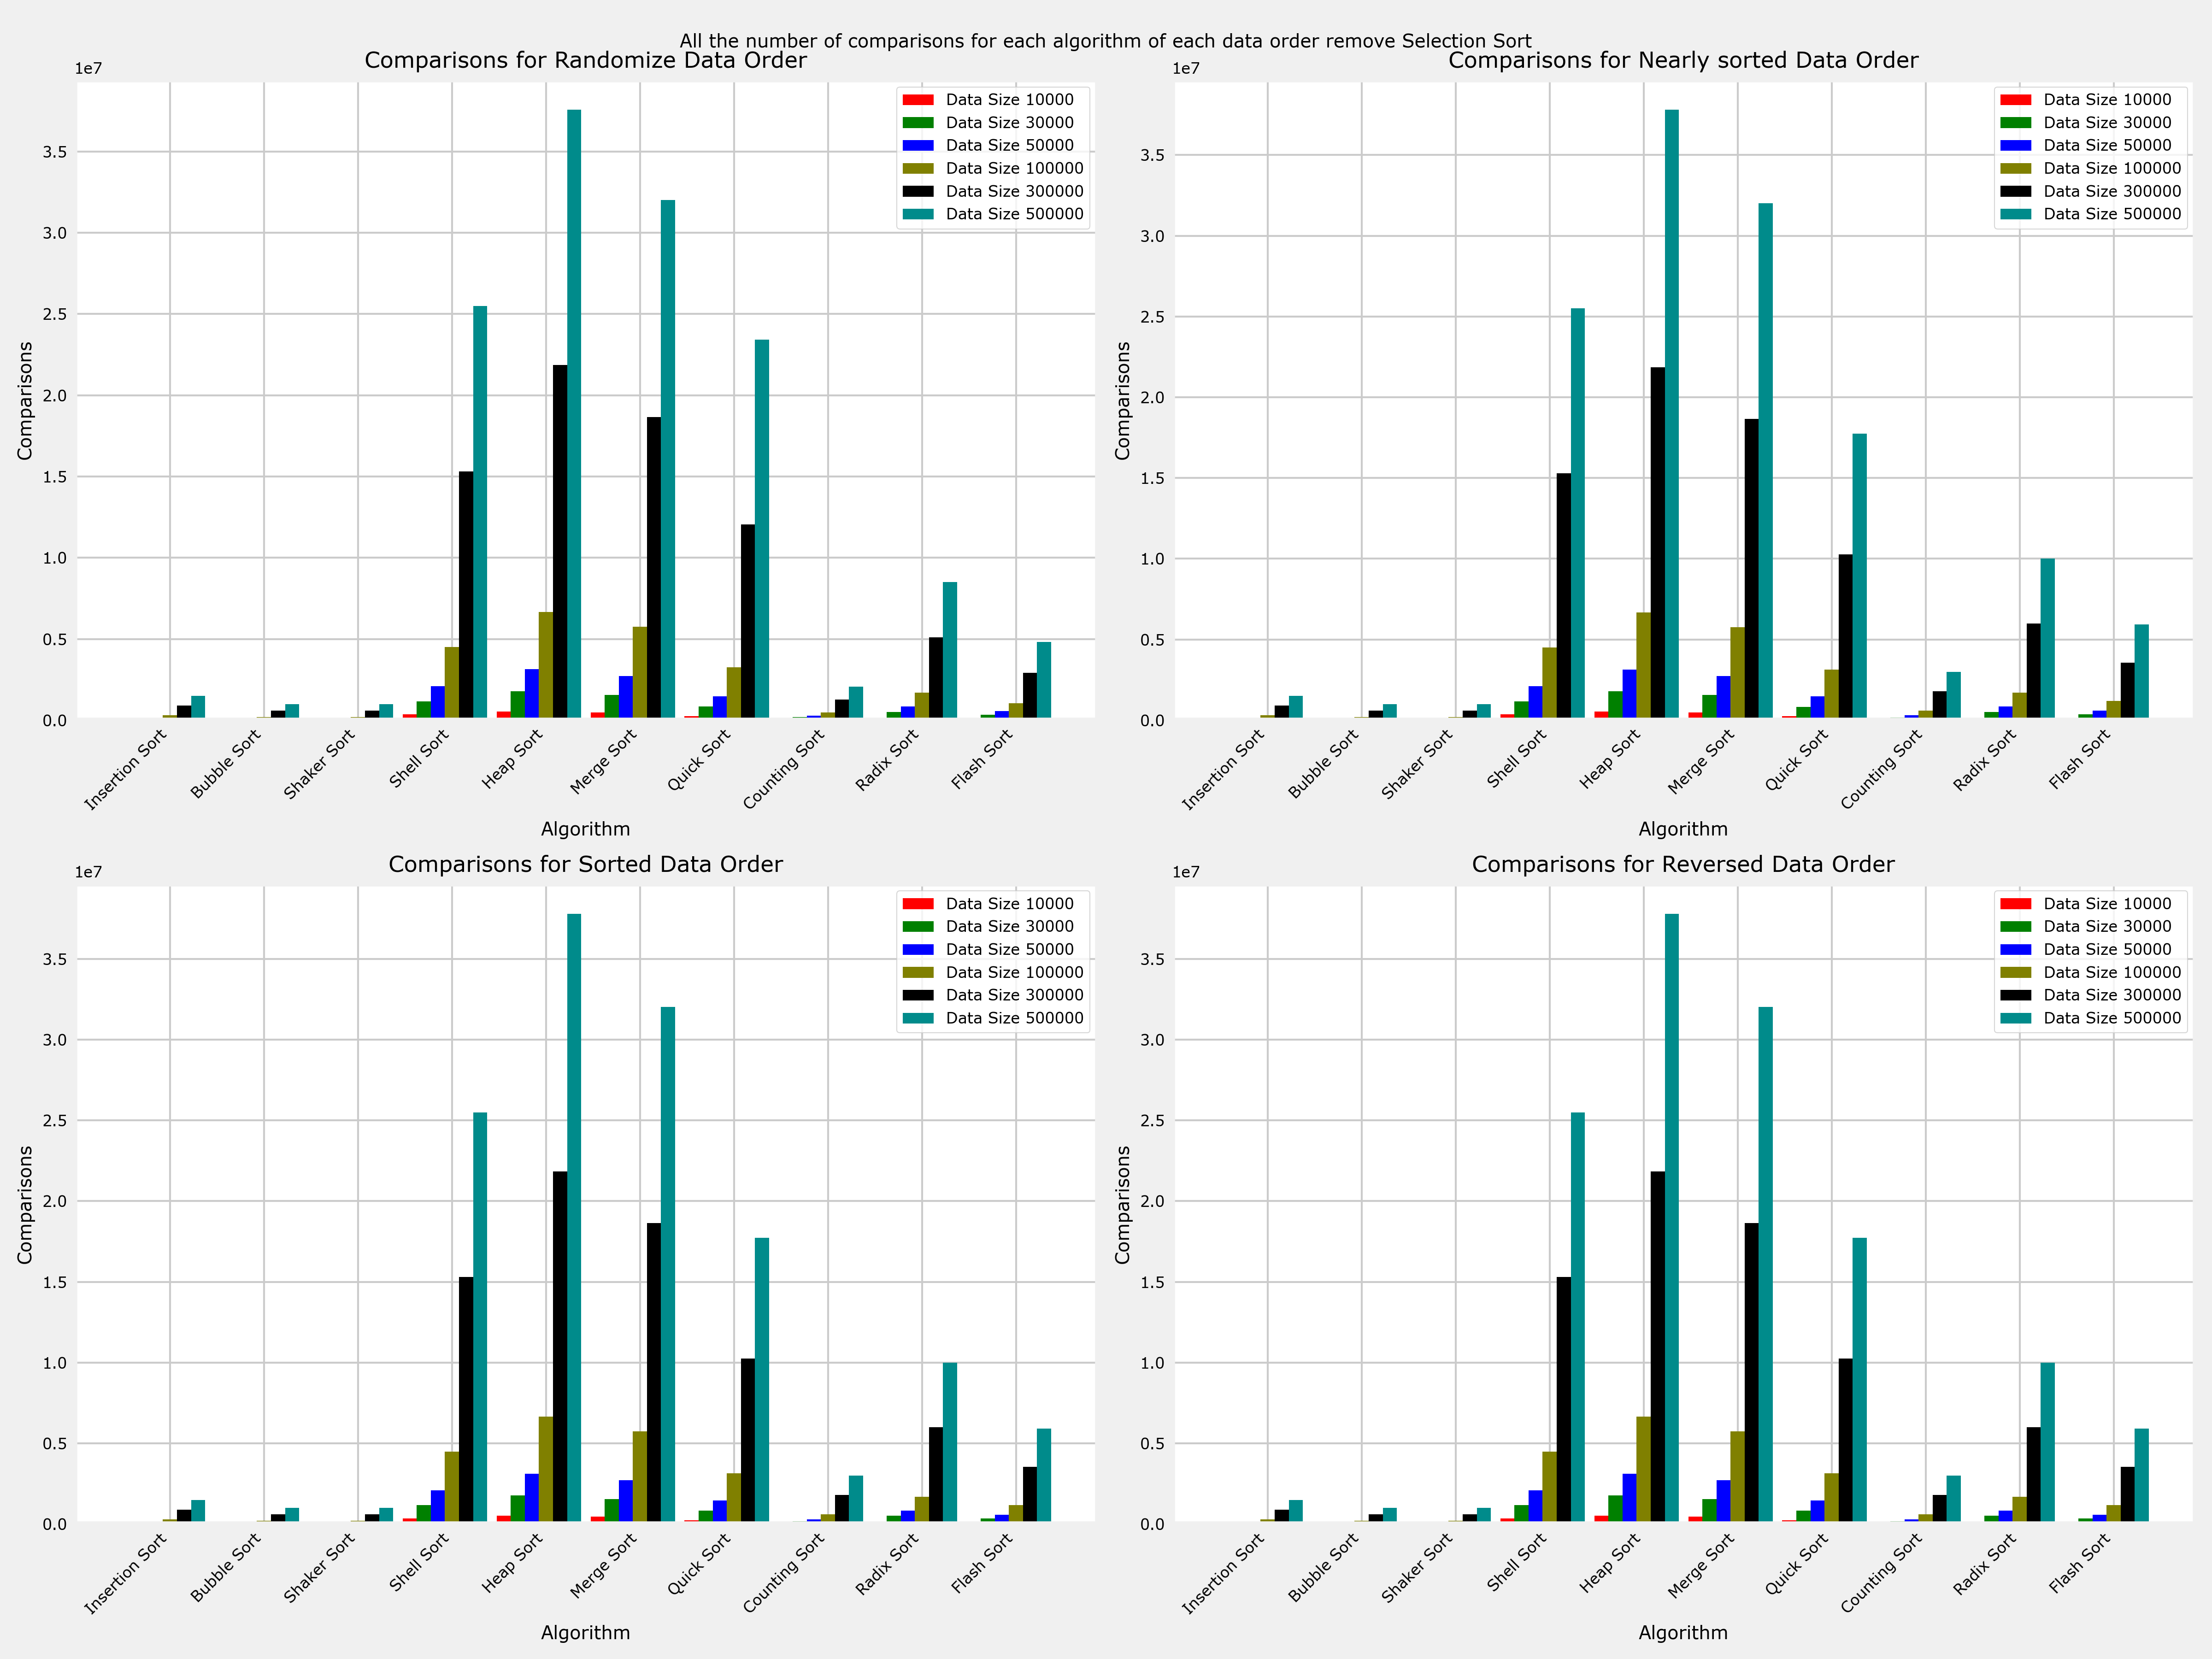
\includegraphics[width=\textwidth]{experimental_result/images/all_the_number_of_comparisons_for_each_algorithm_of_each_data_order_remove_selection_sort.png}
    \caption{Số phép so sánh của 10 thuật toán với tất cả trường hợp của dữ liệu (không có Selection Sort)}
    \label{fig:all_the_number_of_comparisons_for_each_algorithm_of_each_data_order_remove_selection_sort}
\end{figure}


Từ biểu đồ \ref{fig:all_the_number_of_comparisons_for_each_algorithm_of_each_data_order_remove_selection_sort} chia các thuật toán thành 3 nhóm chính: 
\begin{itemize}
    \item Nhóm 1: Insertion Sort, Bubble Sort, Shaker Sort 
    \item Nhóm 2: Shell Sort, Heap Sort, Merge Sort, Quick Sort
    \item Nhóm 3: Counting Sort, Radix Sort, Flash Sort
\end{itemize}

Nhóm 1 có số lượng phép so sánh ít nhất trong tất cả trường hợp của dữ liệu. Ngược lại, nhóm 2 lại có số phép sánh nhiều nhất trong ba nhóm. Điều này có thể là do các thuật toán nhóm 2 cần phải đưa ra quyết định nhiều dựa trên mảng đầu vào. Trong khi đó nhóm 1 và 3 có logic xử lý đơn giản hơn so với nhóm 2.

Tiến hành nhìn kĩ hơn vào từng nhóm thuật toán.

\begin{figure}[H]
    \centering
    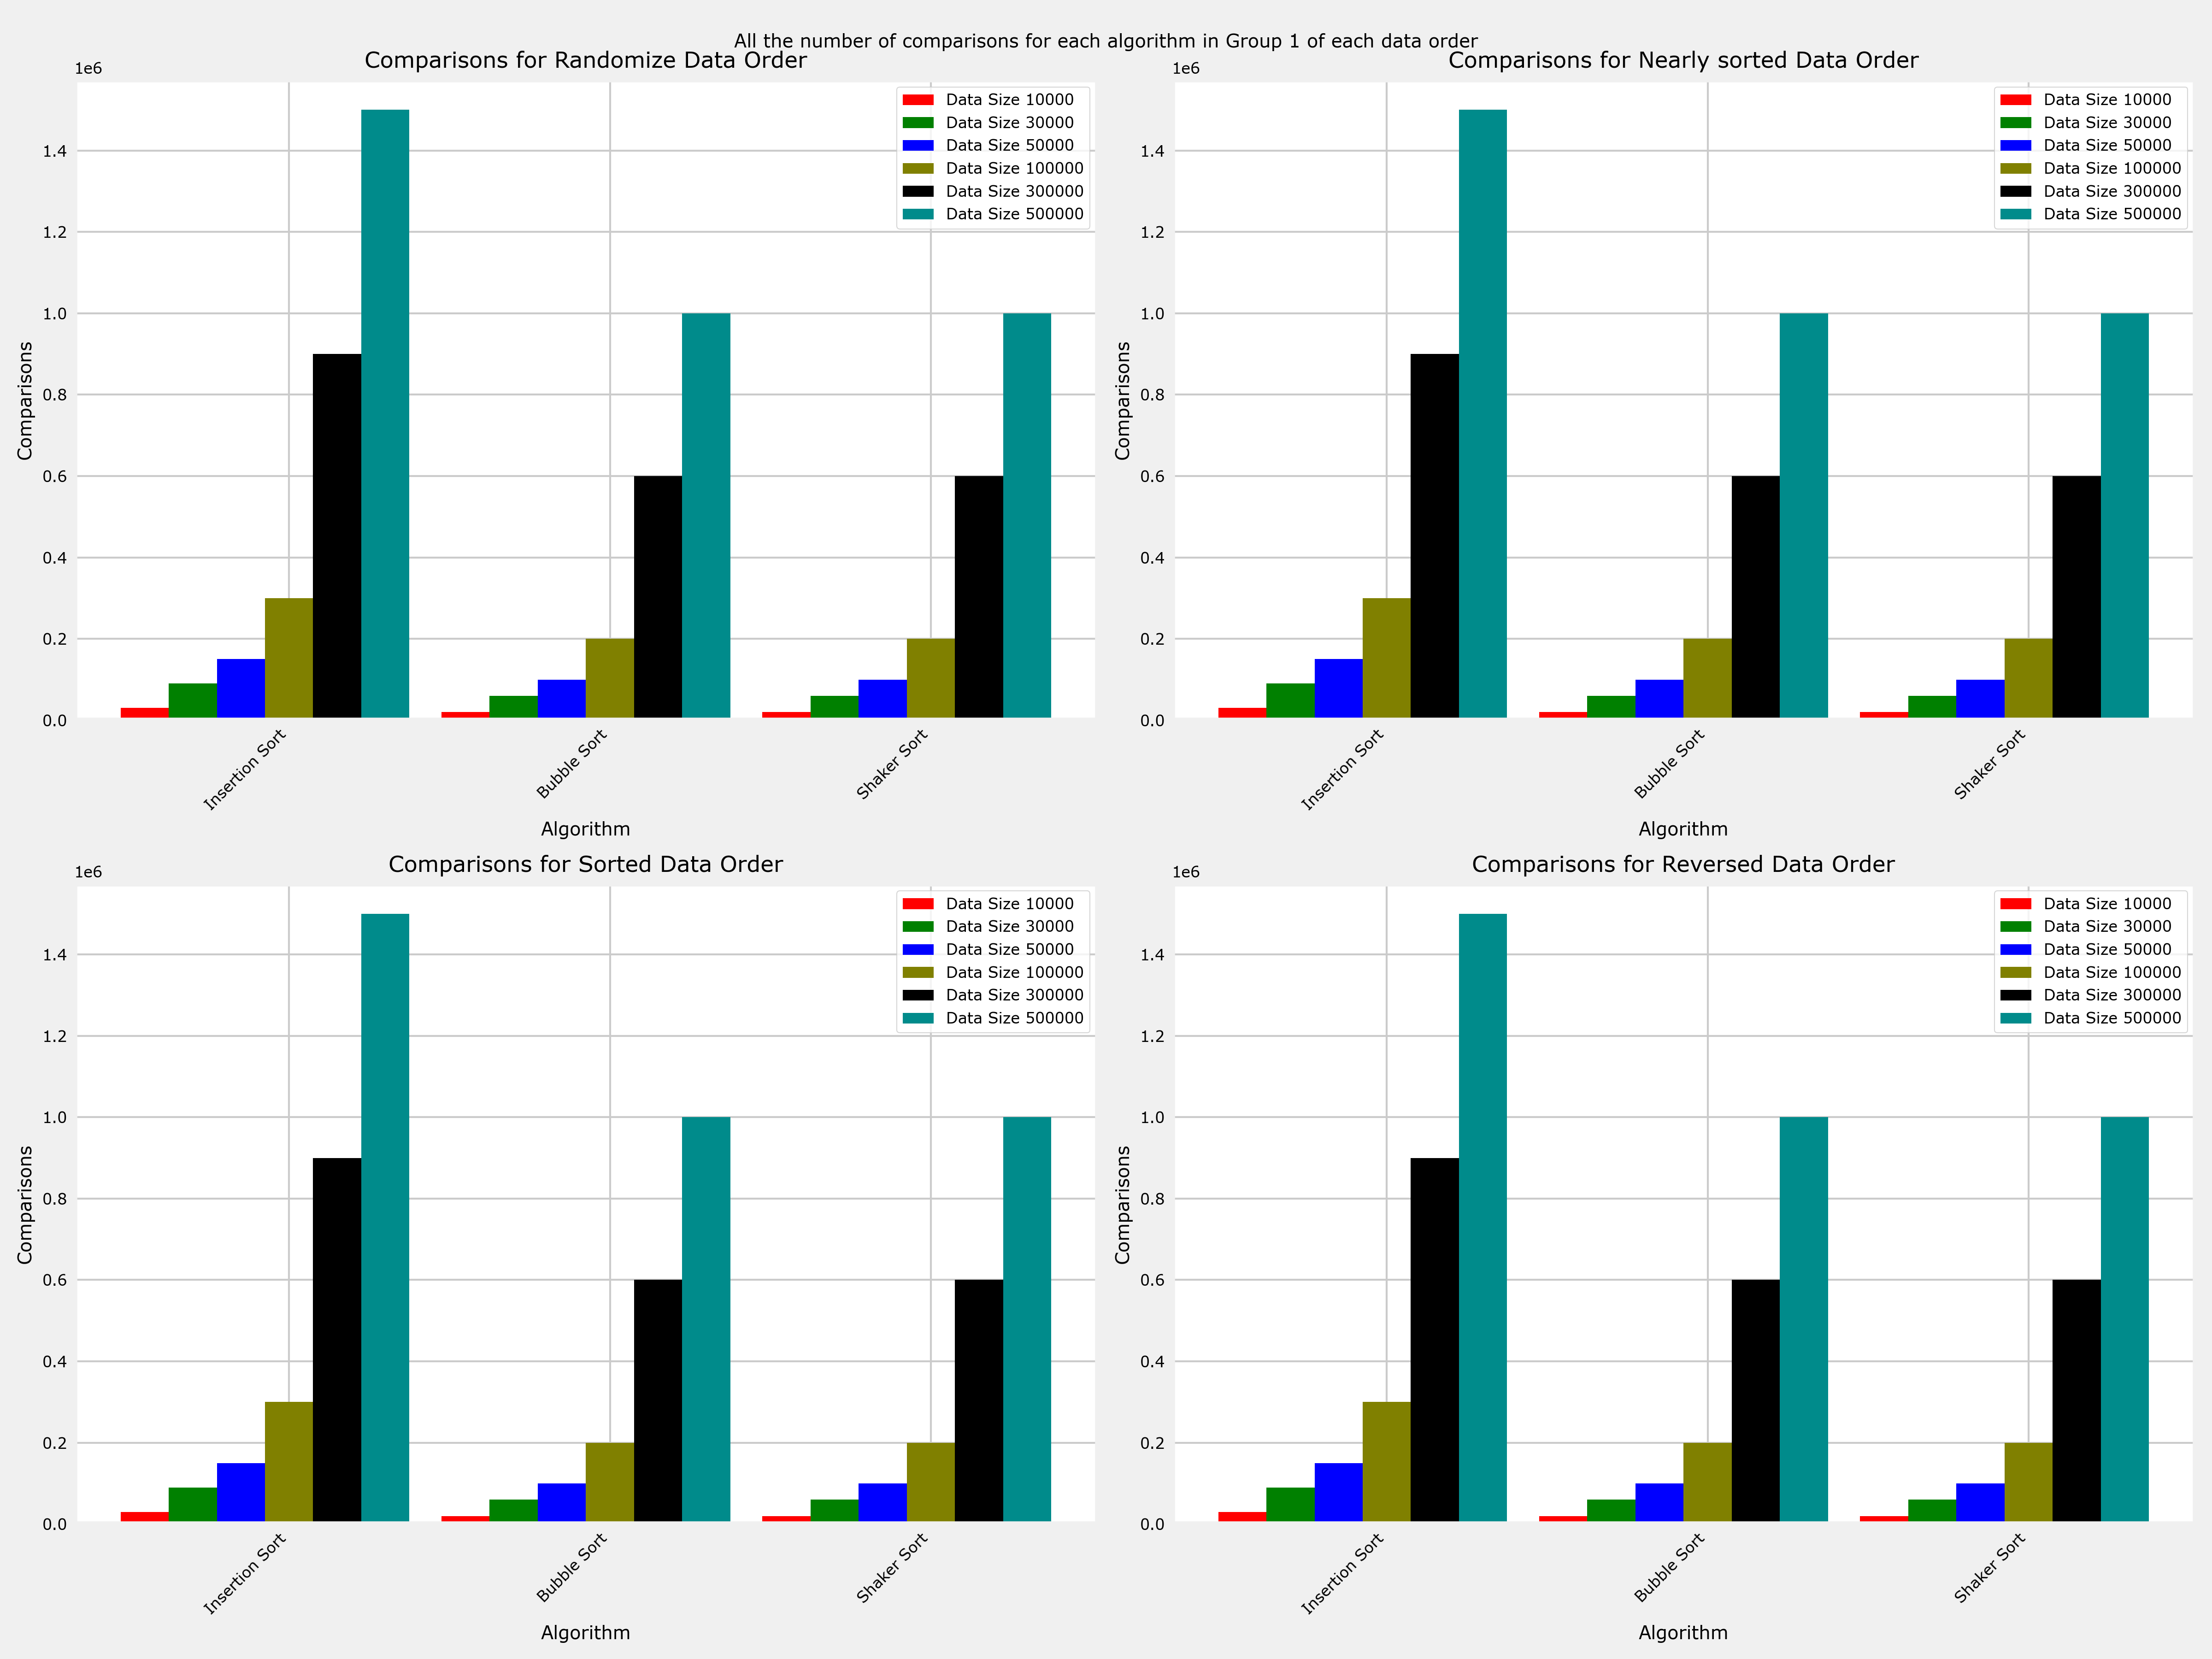
\includegraphics[width=\textwidth]{experimental_result/images/all_the_number_of_comparisons_for_each_algorithm_in_group_1_of_each_data_order.png}
    \caption{Số phép so sánh của Insertion Sort, Bubble Sort, Shaker Sort với tất cả trường hợp của dữ liệu}
    \label{fig:all_the_number_of_comparisons_for_each_algorithm_in_group_1_of_each_data_order}
\end{figure}

\textbf{Nhóm 1}

Theo hình \ref{fig:all_the_number_of_comparisons_for_each_algorithm_in_group_1_of_each_data_order}, ngoại trừ Insertion Sort có độ phức tạp thời gian $\Theta(n)$ trong trường hợp mảng đã sắp xếp, các thuật toán nhóm này đều có xu hướng tăng theo hàm đa thức bậc hai. Điều này do các thuật toán này đều có độ phức tạp thời gian là hàm đa thức bậc hai cho trong hầu hết các trường hợp. 



\begin{figure}[H]
    \centering
    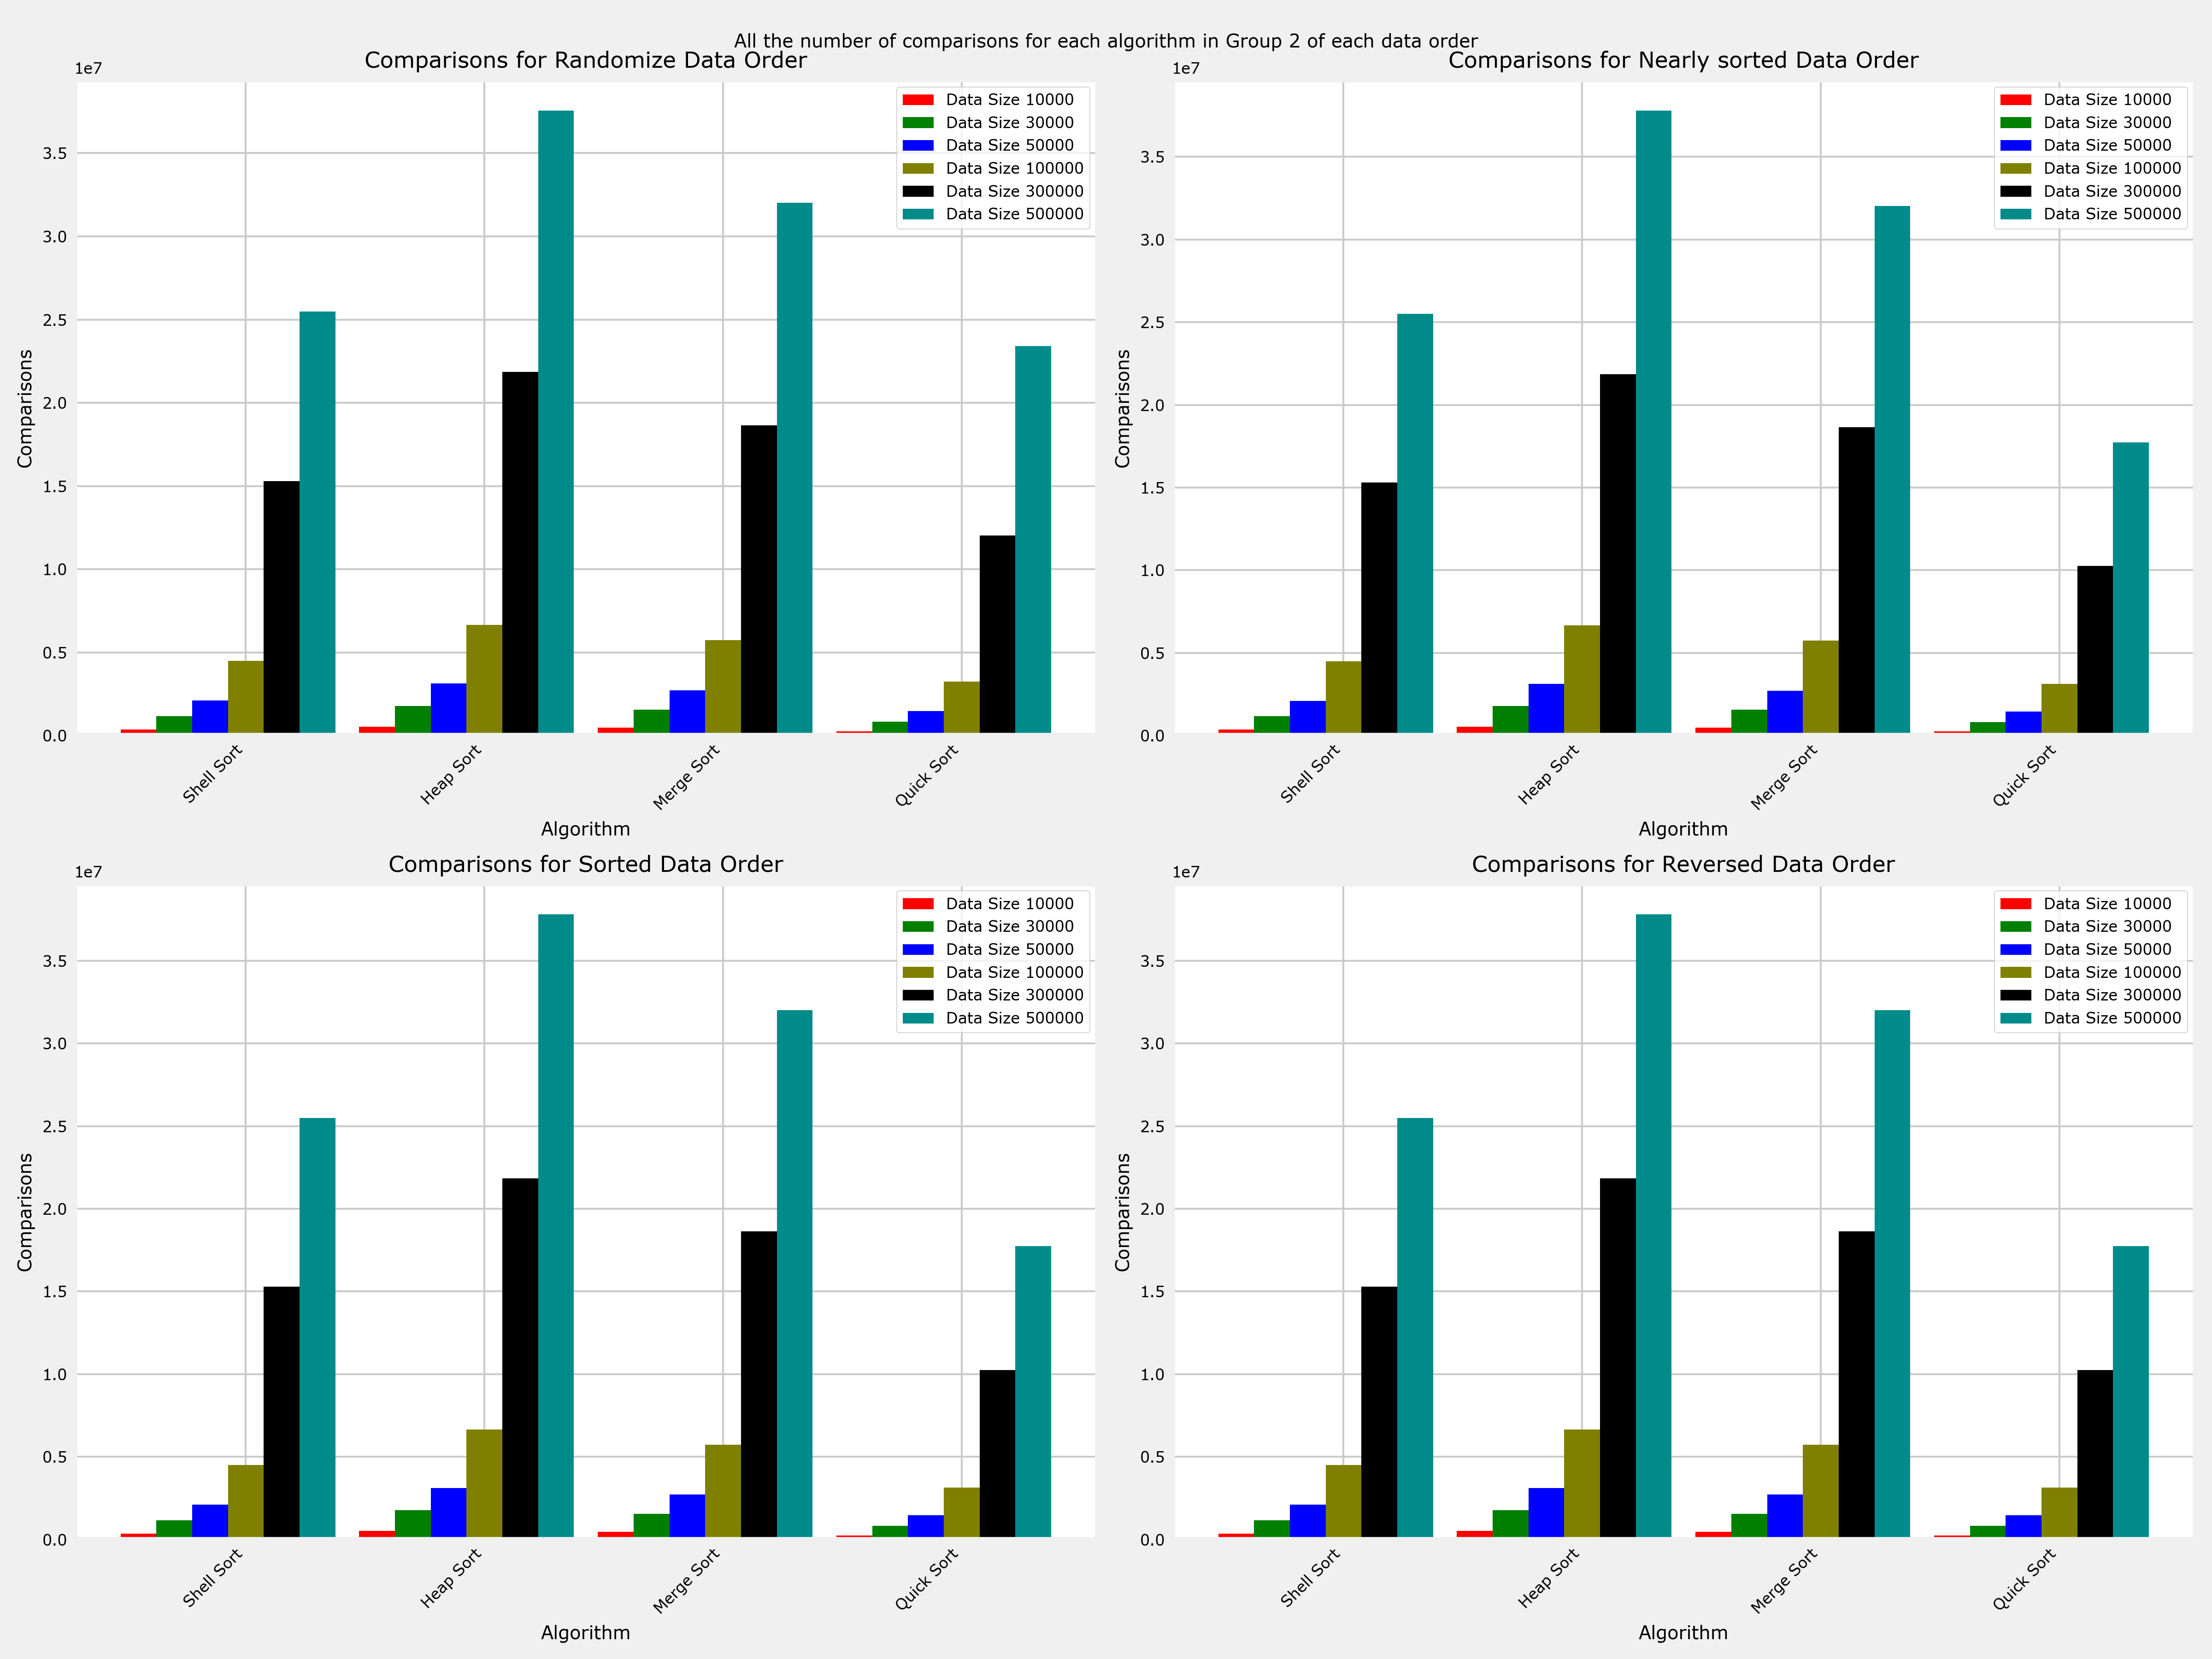
\includegraphics[width=\textwidth]{experimental_result/images/all_the_number_of_comparisons_for_each_algorithm_in_group_2_of_each_data_order.png}
    \caption{Số phép so sánh của Shell Sort, Heap Sort, Merge Sort, Quick Sort với tất cả trường hợp của dữ liệu}
    \label{fig:all_the_number_of_comparisons_for_each_algorithm_in_group_2_of_each_data_order}
\end{figure}

\textbf{Nhóm 2}

Đến với nhóm 2 (hình \ref{fig:all_the_number_of_comparisons_for_each_algorithm_in_group_2_of_each_data_order}), số lượng phép so sánh của các thuật toán này không có hầu như không có sự thay đổi khi đi qua tất cả trường hợp của dữ liệu. Heap Sort có số lượng phép so sánh lớn nhất trong nhóm này, và thấp nhất là Quick Sort. 




\begin{figure}[H]
    \centering
    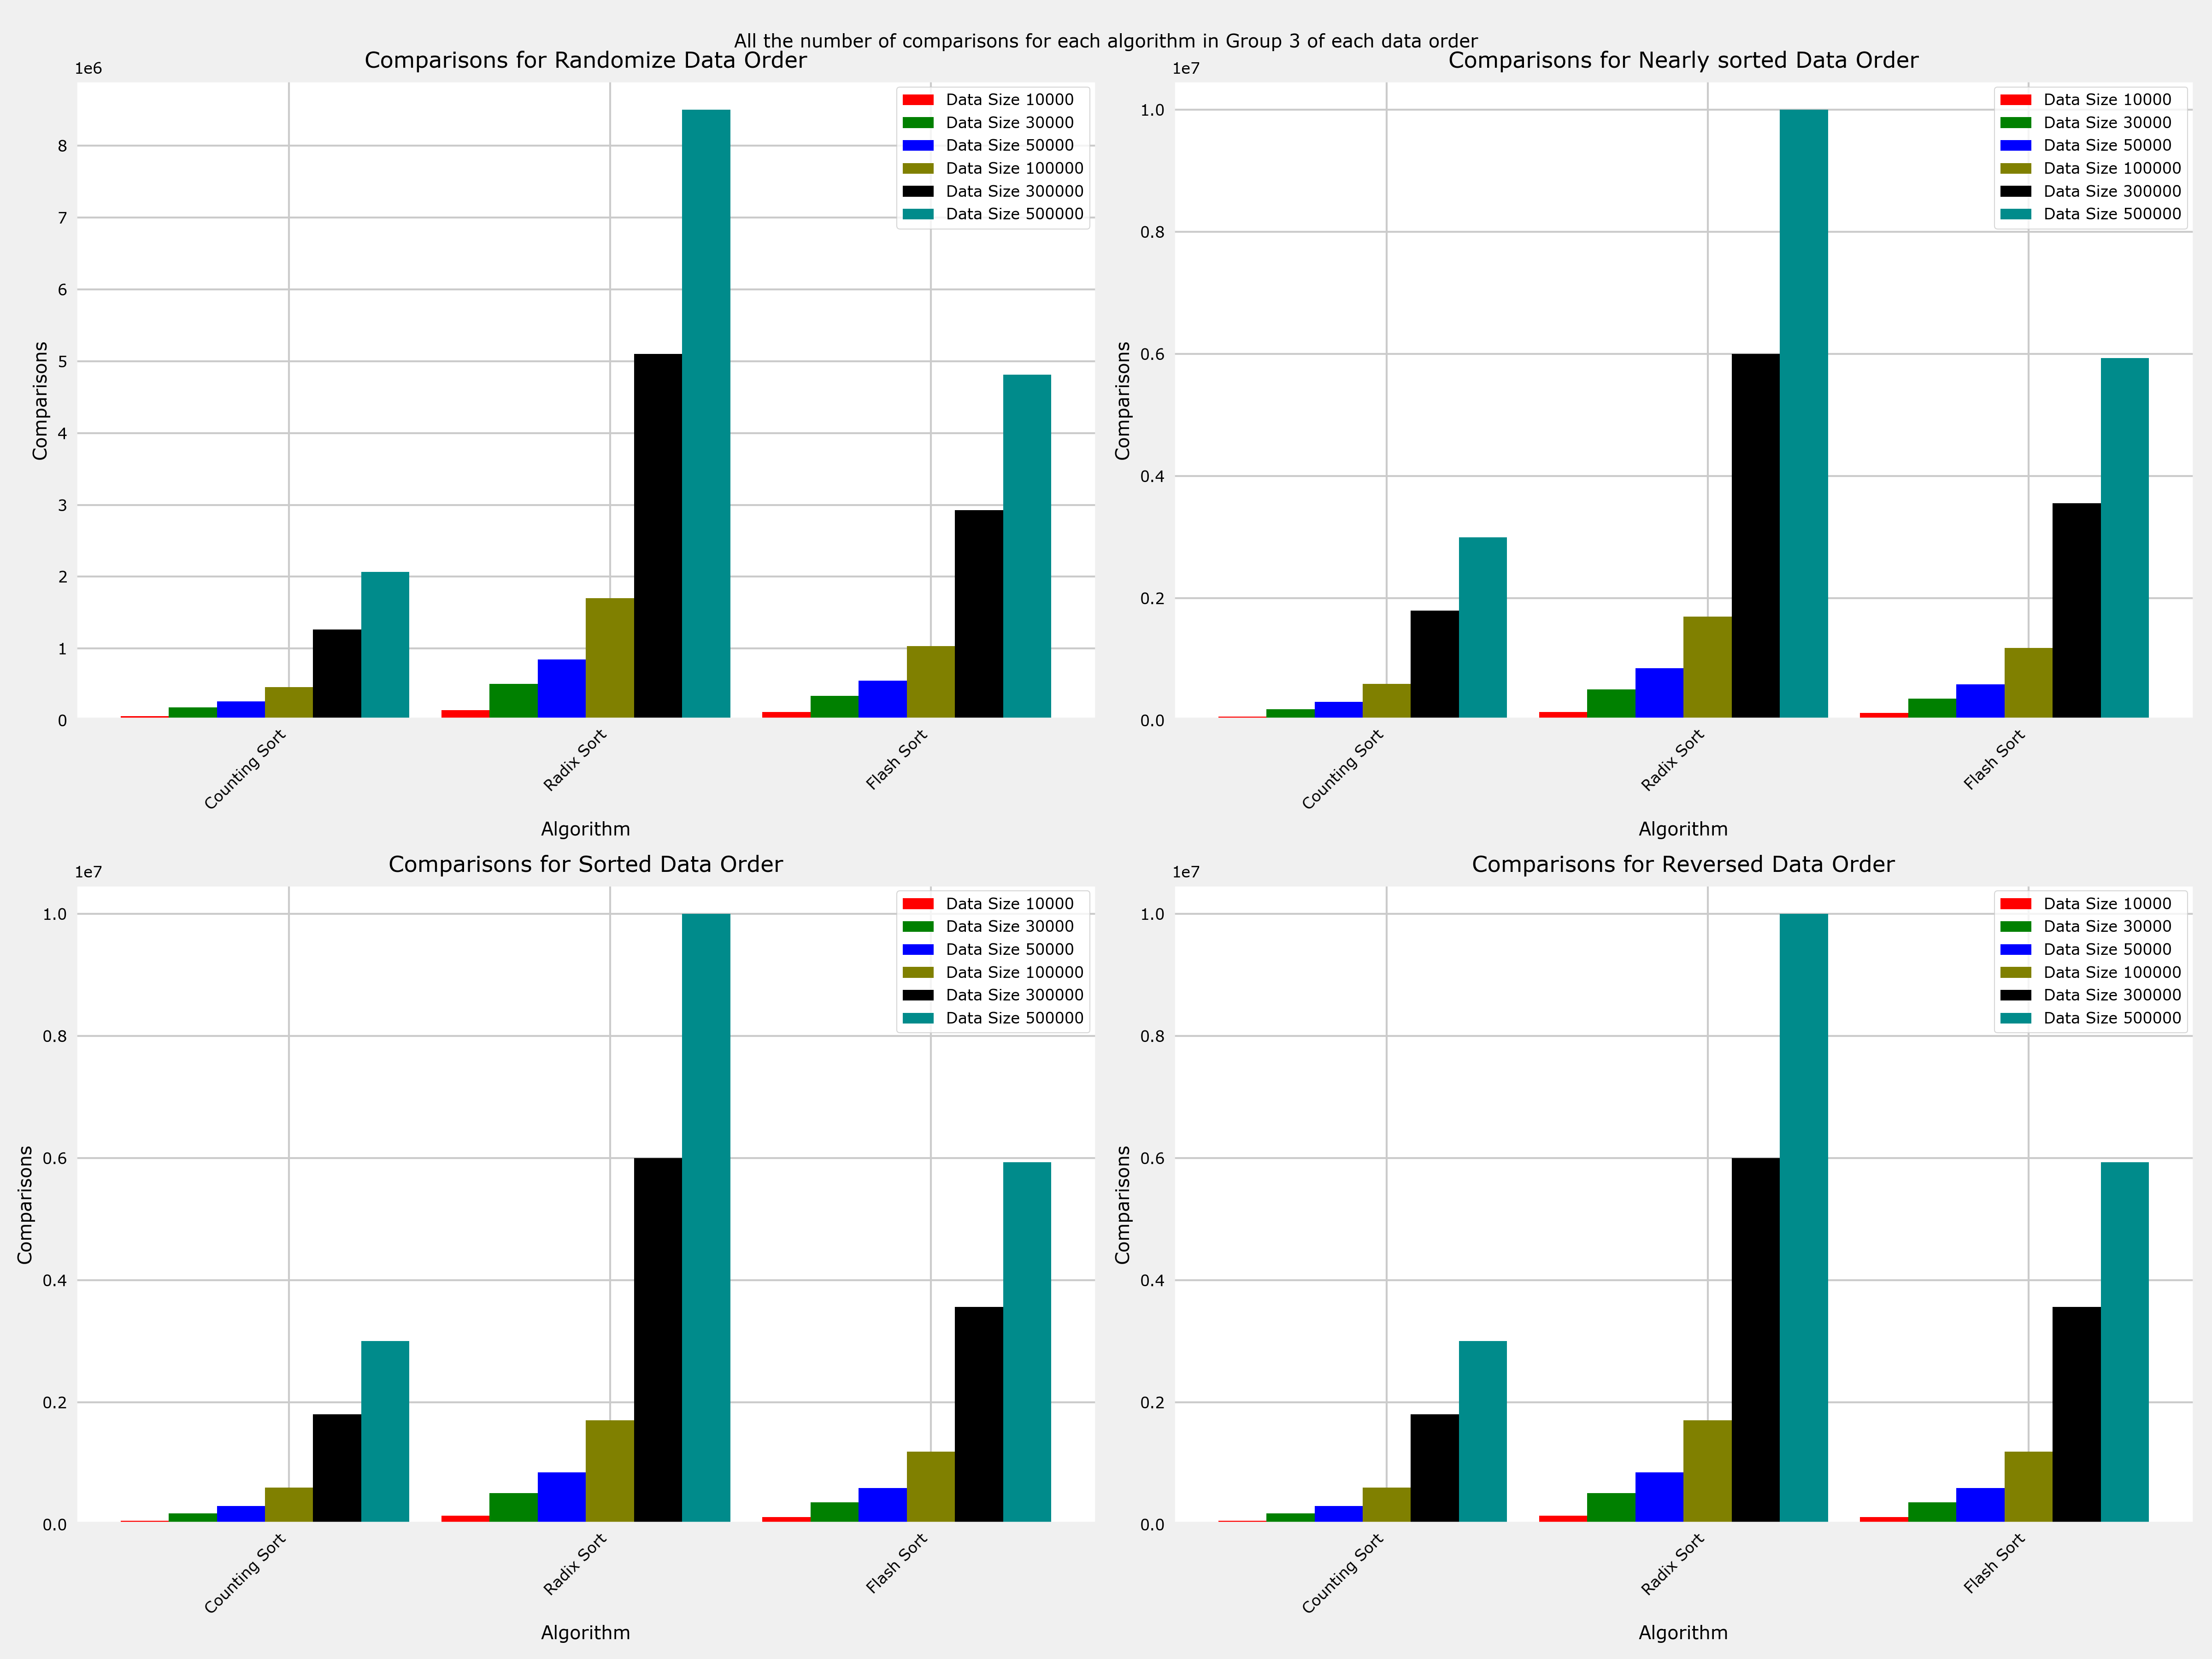
\includegraphics[width=\textwidth]{experimental_result/images/all_the_number_of_comparisons_for_each_algorithm_in_group_3_of_each_data_order.png}
    \caption{Số phép so sánh của Counting Sort, Radix Sort, Flash Sort với tất cả trường hợp của dữ liệu}
    \label{fig:all_the_number_of_comparisons_for_each_algorithm_in_group_3_of_each_data_order}
\end{figure}

\textbf{Nhóm 3}

Counting Sort thể hiển sự vượt trội của mình trong tất cả trường hợp trên hình \ref{fig:all_the_number_of_comparisons_for_each_algorithm_in_group_3_of_each_data_order}, có độ tăng của số lượng phép so sánh khá thấp. Radix Sort có số phép so sánh nhiều nhất trong nhóm này. Flash Sort có số phép so sánh khá ổn định, có thể do sử dụng hàm \textbf{srand} để tạo ra dữ liệu chưa thật sự ngẫu nhiên.
